\documentclass{article}[12pt]
\usepackage{geometry}[top=1in, bottom=1in, left=1in, right=1in, letterpaper]
%\pagestyle{headings}

\usepackage{amsmath}
\usepackage{amssymb}
\usepackage{color,soul}
\usepackage{graphicx}
\usepackage{subfig}

%\title[Author Response: IEEE TCNS : Number 20-0017]{Author Response: IEEE TCNS : Number 20-0017 \\
%\small{Online Synthesis for Runtime Enforcement of Safety in Multi-agent Systems}}

\title{Author Response: IEEE TCNS : Number 20-0017 \\
\small{Online Synthesis for Runtime Enforcement of Safety in Multi-agent Systems}}
\date{}

\begin{document}

\maketitle

\section{Overview}

We would like to thank all the reviewers for their time and valuable feedback for this submission. The implemented modifications to the manuscript are shown in blue colored font in the new submission. 

In particular, we modified the organization of section III. As per the suggestion of reviewer~11, the examples (now called scenarios) appear after the problem statement. We rewrote the definitions of the properties of the enforcers in the theorem environment. Additionally, as suggested by reviewer~6, we added references for the notations used. We cited and compared some of the existing approaches for collision avoidance. Based on the suggestion by reviewer~7, we provided a toy grid world example to demonstrate the working of the ordering mechanism when the agents are in different communication groups.

We make more modifications in different sections in response to the specific suggestions from reviewers. Next, we go into detail and respond directly to each comment. The reviewer comments have been highlighted in yellow. Our answers are written in plain text.

\section{Review 27475 (Reviewer 6)}

\begin{enumerate}

\item  \hl{Page 2, Right column, please provide some more references for the preliminaries. Many uncommon nations are used in this section that are not described or explained very well.}

In page 2, right column, we added references for the notation. The notations we use are adopted from the fields of runtime enforcement and formal methods in computer science. The references are listed below. 

\begin{itemize}
\item “Runtime enforcement monitors: composition, synthesis, and enforcement abilities”~\cite{Falcone2011}.
\item “Synthesizing enforcement monitors w.r.t.~the safety-progress classification  of  properties”~\cite{falconeruntime1}.
\item “Runtime enforcement of reactive systems using synchronous enforcers”~\cite{Pinisetty2016runtime}.
\end{itemize}

Additionally, for graph theoretic concepts (for example labeled graphs) we adopt the definitions and notations from the textbook``Introduction to Graph Theory''~\cite{west_introduction_2000}.

\begin{enumerate}
\item  \hl{First, the authors defined $\mathcal{U}$ as a set of node labels, later $\mathcal{U}$ is applied as the set of agents. Please provide more relationship between them.}

In page 3, we added a clarification that the set of node labels is the same as the set of all agents. %The labels that currently hold at a location indicate which agents are occupying that location.
Formally, at time $t \in \mathcal{T}$, an agent $u$ is said to be at location $v$ if $u \in \chi(v,t)$. More than one agent can be at the same location at a given time. 

\item  \hl{Please describe the notations $2^U$ and $2^V$ more clearly. This notation is not common. The authors are suggested to provide some references about these notations.}

If $A$ is a set, then $2^A$ is the power set. We added this clarification and provide citations for the used notations in section II (see answer to question 1).

\item  \hl{When the time variable is defined, the time domain should be explicated, e.g., $t \in \mathbb{T}$. Furthermore, it should be emphasized that in this paper a discrete time system is considered.}

We added the domain and emphasized the discrete nature of time. 

\item \hl{What is the meaning of $w[i : \ell]$? In the manuscript, $w = a_1a_2 \dots a_n$ and $w = w_0w_1w_2 \dots$. What is the index of the first element, 0 or 1?}

This error is a typo. We fixed the index of the first element to be 0.

\item \hl{What is the difference between $\Pi_i(e)$ and $\Pi_i~e$?}

This error is a typo. $\Pi_i~e$ is the correct notation.

\end{enumerate}

\item \hl{Page 3, Left column, the notation $s$ denotes an action and a label. What is the difference between them?}

Analogously to the node labeling, the edge labels denote the available actions to agents. In page 3, we add the clarification that the set of actions available to the agents is the set of edge labels. 

\item \hl{Page 3, Left column, in the sentence, then at time $t + i, (i \leq w)$, what is the domain of the variable i? Is it a label, agent, or time?}

The variable $i$ is an integer. We mention this explicitly and also change $w$ to $|w|$. 

\item \hl{Please provide a number for every equation, especially for the equation that is mentioned in the text.}
	
We added equation numbers to all equations.

\item \hl{Page 3, Left column, Associated with after the equation should be revised as associated with.}
	
On page 3, we added a period after the equation.

\item \hl{Page 3, Left column, what do the notations $\{\ell, r, t, d\}$ stand for?}

On page 3, we added an explanation that these actions correspond to moving left, right, top and down, respectively.

\item \hl{Page 3, Left column, in the sentence, The state of the blue agent is (2, 1) and the green agent is (2, 1)., the first (2, 1) should be (1, 2).}
	
On page 3, we changed “$(2,1)$” to “$(1,2)$”.

\item \hl{Page 3, Right column, the notation $U_i$ should be revised to $U_{u_i}$ according to the previous notations.}

 On page 3, we modified the subscript to $\mathcal{U}_{u_i}$. 

\item \hl{Page 4, Left column, according to the definition of $S_1$ and $S_2$, they are defined on the time domain. But the time domain $T$ is not explicitly shown in the definition.}
	
We modified the notation to clarify the domain and co-domain of $S_1$ and~$S_2$. We use square brackets to denote the agent and time instead of parentheses. 
For example in page 7, we use $S_1[u,t](O,V,W)$ instead of $S_1(u,t)(O,V,W)$.
We propagated this modification throughout the paper. 

\item \hl{Page 10, Right column, in In the second setting shown in 7 (top)..., the word Figure should be added. There is only one figure in Figure 7. What does the word top indicate?}
	
On page 10, this error was a typo. Hence, we removed the “top”.

\item \hl{In Section VI, the proposed approach is applied in the context of collision avoidance for multi-agent systems. It is well-known that repulsive potential force method can be applied to solve the problem of collision avoidance. Therefore, the authors are suggested to compare the novel approach to some existing approaches}~\cite{Zhu2020AdaptiveOD,Zhu2019,Rudd2017,AlAbri2020ADO}.

Thank you for bringing these to our attention. In Section I (introduction), we have added two paragraphs contrasting our technique against some of the existing approaches to collision avoidance. We cite and compare all the suggested works. The main point of contrast is that we provide theoretical guarantees of both completeness and finite-time progress. These guarantees are typically difficult to prove in decentralized, multi-agent systems. We explain in more detail in the following.  

In “Adaptive Online Distributed Optimal Control of Very-Large-Scale Robotic Systems”~\cite{Zhu2020AdaptiveOD} an online reinforcement learning technique is used for path planning. In “Scalable gas sensing, mapping, and path planning via decentralized Hilbert maps”~\cite{Zhu2019}, a discriminative classifier, that is used to map gas distribution, is trained online. Entropy-based artificial potential field and the entropy-based particle swarm optimization algorithms are used in conjunction with the classifier for path planning. In contrast with the above techniques, the method in this paper modifies the trajectories of the agents only when collisions are detected. Additionally, the method guarantees progress, i.e., no single agent keeps deviating continuously to keep the system safe (collision free).

In “A Generalized Reduced Gradient Method for the Optimal Control of Very-Large-Scale Robotic Systems”~\cite{Rudd2017}, a distributed optimal control method based on generalized reduced gradient method is used for path planning; it provides no guarantees for completeness.  In contrast, we ensure a path exists if a centralized planner is able to find a path. More specifically, the technique in this paper, under certain assumptions, will synthesize decentralized enforcers that guarantee safety for all agents if there exists a centralized enforcer (referred to as a shield in~\cite{BharNFM}) that can guarantee safety.

In contrast to “A Derivative-Free Optimization Method With Application to Functions With Exploding and Vanishing Gradients”~\cite{AlAbri2020ADO}, the environment in our problem is a discrete graph, and the agents take one unit of time to move from one node to the other, i.e., the agents have uniform dynamics that do not depend on their location. These restriction enable us to ensure progress and completeness through online synthesis.

\end{enumerate}

\section{Review 27477 (Reviewer 7):}

\begin{enumerate}
\item \hl{As done for the terminologies and different concepts, it will be useful to explain the algorithms using some of the toy grid world examples.}


\begin{figure}[h]
    %\centering
    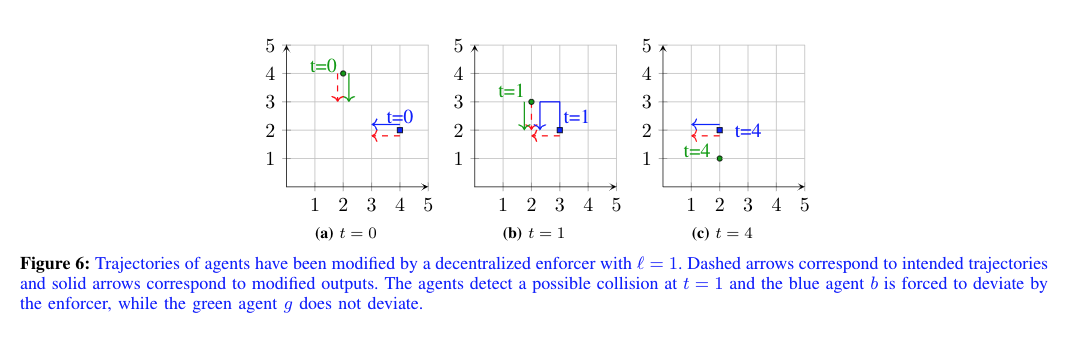
\includegraphics[scale=0.8]{fig6.png}
    \caption{Example to explain the priority exchange algorithm.}
\end{figure}

\iffalse
 \begin{figure}[h]
    \centering
    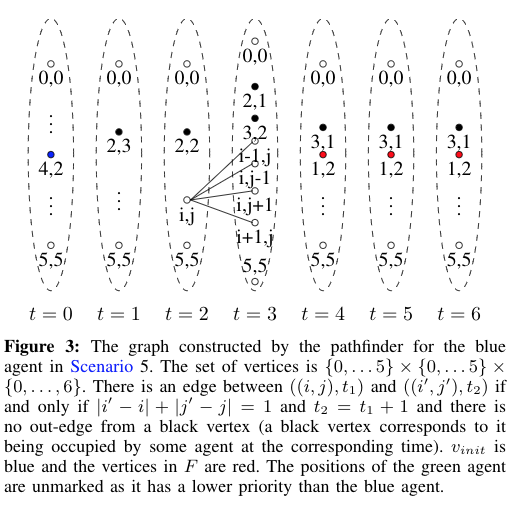
\includegraphics[scale=0.7]{fig3.png}
    \caption{Example to explain the pathfinder.}
\end{figure}
\fi

We explained the priority exchange algorithm using an additional scenario (Scenario~10) and Figure~1 (Figure~6 in paper). See the answer of question~4 for a detailed explanation of use of flags for maintaining the priorities. Scenarios that explain the working of the pathfinder is presented in Scenarios~7 and~8 and Figure~3 (in paper).

\item \hl{ Please provide references to establish the fact that state-of-the-art synthesis time is exponential. }

In general, the optimization of the plans of $n \in \mathbb{N}$ cooperative robots is known to be PSPACE-hard problem  ``Elias  Xidias,  P.  Zacharia,  and  Andreas  Nearchou: Path  planning  and scheduling for a fleet of autonomous vehicles" \cite{hardness}. Therefore, it is not surprising that most known algorithms run in exponential time. In section VI, we add this reference.

\item \hl{In example 1, labeling function for blue agent at $t=1$ should be $\chi((3,2),1)$ right? In example 6, is the communication radius still 2?}

Yes, this is true. In addition, in example 6 (now scenario 6) we explicitly state the communication radius.

\item \hl{The local ordering strategy between two agents is percolated throughout the network in a hierarchical manner to show that the global ordering for an arbitrary number of agents remains consistent. While it is clear mathematically, an example with multiple communication clusters would be useful to explain this idea further. }

We provide an Example (see Figure 6) to demonstrate the working of the flags. More specifically, we consider the case when the $\ell=1$ and $d=1$. 
Initially, the two agents are in different communication groups and $b \prec_0 g$ (green agent has precedence over the blue agent). At $t=1$, the two agents are in the same communication group. Therefore, the flags $B_b$ and $B_g$ are updated. More specifically, $B_{b} = \{g\}$, $B_{g} = \{b\}$ and the flags $c_b^g = c_g^b = 0$, i.e., none of the agents have reached a goal after communicating with the other agent. At $t=4$, the green agent has reached the goal. Therefore, $c_g^b=1$, this implies $g \prec_4 b$.  At $t=5$, the blue agent reaches it goal, therefore $c_b^g =1$, which implies $b \prec_5 g$. Lastly, both $c_b^g$ and $c_g^b$ are reset to~$0$.

%\textcolor{blue}{{\textbf{Can you actually explain it here?}}}

\item \hl{Please provide a discussion on how real life communication drop/delay/errors may impact the online synthesis strategy. Basically is there a notion of robustness?}

This is an excellent point. We do not address the issue of communication loss in this paper. Moreover, we have assumed perfect and instantaneous communication between agents. In the future, we will aim to try to relax this assumption. For example, we are interested in studying the effects of intermittent communication loss and the cases in which we can still provide theoretical safety guarantees. 
We modify the Conclusion saying that dealing with communication losses is a future direction.

\item \hl{Please provide a discussion on how the analysis and the corresponding bounds may change for a higher dimensional action space, i.e., when agents have many more possible actions available at every step. }

The pathfinder has to find new (safe) trajectories of size $\ell + k$. The pathfinder performs a localized graph search based on the look-ahead $\ell$ and the permitted deviation size $k$. Hence, the complexity of finding a safe trajectory depends only on the number of agents $|\mathcal{U}|$, $k$ and $\ell$ and does not depend on the size of the environment as proved in Theorem 2. We have provided a formal remark after the proof of Theorem 2 on page 8.

\end{enumerate} 

\section{Review 28275 (Reviewer 11)}

\subsection*{Section 3}

\begin{itemize}

\item \hl{Placement of subfigures in Figure 1 is quite confusing. Figure 1b is referenced in Example 1 and Figure 1a is referenced in Example 2.}

In Figure 1, we changed the order of the figures and the corresponding caption.
 
\item \hl{I suggest setting up the problem in the beginning of Section III, and then exploring various scenarios to improve the reading. The word Example may be replaced by Scenario.}
	
We restructured section III as suggested. Now, we first introduce the concepts required for setting up the problem and then set up the problem. We provide the examples (now called scenarios) after setting up the problem.

\end{itemize}

\subsection*{Section 4}

\begin{itemize}
   
\item \hl{In section IV, it is not clear whether the pathfinder is globally accessible or only locally available.}

The pathfinder for any agent is accessible only to that agent. In section~IV, we now restate it for clarification. 

\item \hl{The reason for Assumption 1 is not stated. I suspect Assumption 1 allows the agent to stay idle at its current location. Please add a few descriptive lines to this effect.}

Yes, in fact the self-loops allow the agents to idle. We added this clarification.

\item \hl{The sentence ``In contrast, here is a partial function S1 which is when required.'' on page 7 is nonsensical. }
	
In section IV, in the corresponding line, we had missed a “constructed”. The new sentence is “In contrast, here is a partial function S1 which is constructed when required.”

\item \hl{ The proof of the main theorem (Theorem 1) of the paper is not really a proof. For example, the second last line states that an enforcer can ensure safety if some shield can ensure safety. The assumption that some shield can ensure safety is not made anywhere in the statement of the theorem. Further, the phrase deviate minimally is not well defined. Is the minimal deviation unique?}
\hl{Are their paths that are equivalently minimal?} \hl{It seems that the most trivial solution can be obtained when an agent is allowed to move only in the case where the agent with the next higher priority reaches its goal. This policy will trivially avoid all collisions without any modification to any agent's trajectory. It is also not clear whether the total time is bounded. }
\begin{figure}[h]
    \centering
    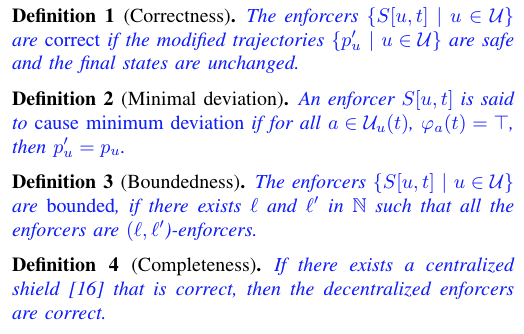
\includegraphics[scale=0.9]{defns.png}
\end{figure}

In section III, we now use the theorem environment for the definitions of the enforcer properties. 
By the new definition of minimal deviation, the confusion regarding the uniqueness etc. is removed. We refer to these definitions in the proof of Theorem 1. Essentially, the proof of Theorem~1 is a direct consequence of the lemmas preceding it. Lastly, the trivial solution where the agents wait until the current highest priority agent reaches the goal is now invalid (it will violate minimal deviation).

\end{itemize}

\subsection*{Section 5}
\begin{itemize}
\item \hl{The second paragraph is missing a verb in the sentence ``$w_u (0)$ be the trajectory (possibly infinite) for agent u.''}

We fix the sentence grammatically by adding “Let”. 
\end{itemize}

\subsection*{Section 6}

\begin{enumerate}

\item \hl{In the Gazebo simulation, is the world a discrete grid? If yes, what is the size of the grid. If no, how is the continuous space discretized to use the method developed in this paper to enforce constraint?}

Yes, in the Gazebo simulation, the world is a discrete grid. We discretize the grid such that the transition of each vehicle from one cell to another cell is synchronized and timed. That is, when a vehicle is assigned its next target cell, it transits to such a cell and waits until all the other vehicles reach their target (for the same time step) before receiving a new target cell. 
We explained the discretization in the body of section VI.

\item \hl{Instead of videos, plots showing the flag switching times as the agents modify their trajectory might be more suitable for reproducibility.}

\begin{figure}[h]
    \centering
    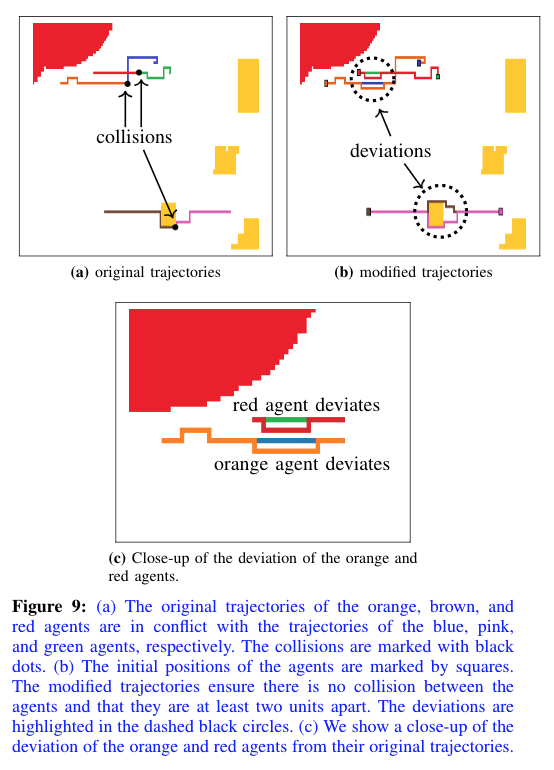
\includegraphics[scale=0.8]{fig9.png}
\end{figure}

In page 11, we added plots for the original and modified trajectories of the agents (Figure 9). In addition, we also highlight the modifications.
%We provide links to data files for the trajectories and the obstacles.

\end{enumerate}

\bibliographystyle{unsrt}
\bibliography{ref}

\end{document}